\documentclass[landscape,a5paper]{article}
\usepackage[utf8]{inputenc} 
\usepackage[usenames,dvipsnames]{xcolor}
\usepackage{fullpage}
\usepackage{tkz-graph}
\thispagestyle{empty}

\topskip
\footskip

\begin{document}
\vspace*{\fill}
\begin{center}
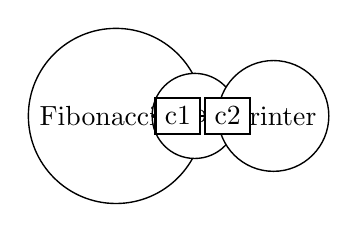
\begin{tikzpicture}[node distance   = 4 cm]
     \GraphInit[vstyle=Normal]
     \tikzset{LabelStyle/.style =   {draw}}
     \Vertex{FibonacciInt}
     \EA(FibonacciInt){Stop}
     \EA(Stop){Printer}
     \tikzstyle{EdgeStyle}=[->]
     \Edge[label=c1](FibonacciInt)(Stop)
     \Edge[label=c2](Stop)(Printer)
  \end{tikzpicture}
\end{center}
\vspace*{\fill}
\end{document}
